\documentclass[11pt]{article}
\usepackage[margin=1in]{geometry} 
\usepackage{amsmath}
\usepackage{tcolorbox}
\usepackage{amssymb}
\usepackage{amsthm}
\usepackage{commath}
\usepackage{lastpage}
\usepackage{fancyhdr}
\usepackage{accents}
\usepackage{csquotes}
\usepackage{soul}
\newcommand{\ubar}[1]{\underaccent{\bar}{#1}}
\pagestyle{fancy}
\setlength{\headheight}{40pt}


\newenvironment{solution}
  {\renewcommand\qedsymbol{$\blacksquare$}
  \begin{proof}[Solution]}
  {\end{proof}}
\renewcommand\qedsymbol{$\blacksquare$} % add packages, settings, and declarations in settings.tex

\begin{document}

\lhead{Yida Liu} 
\rhead{EECS 416 Spring 2020 \\ Convex Optimization for Engineering \\ Homework 1} 
\cfoot{\thepage\ of \pageref{LastPage}}

\textit{All screenshot of excel are attached.}

\section{Minimize Inscribed Triangle Perimeter} \label{prob1}

First, we revisit the definition of linear interpolation between two points. As from the Wikipedia page:
\begin{displayquote}
linear interpolation is a method of curve fitting using linear polynomials to construct new data points within the range of a discrete set of known data points.
\end{displayquote}
We define this function $$I(M, N, t)= tM + (1 - t)N$$where $M$ and $N$ are coordinates (in this case, in $\mathbb{R}^2$), $t\in[0, 1]$. Function $I$ gives a new coordinate in the straight line between M and N depending on the value of parameter $t$. Now we shall begin the formulation of the model. 

For this problem, we would like to find the location of points D, E, F lies on line AB, BC, AC in acute triangle ABC such that the new triangle DEF has minimal perimeter.

Above definition clearly suggests that the location of D, E, F can be expressed in terms of the linear interpolation of AB, BC, and AC. Hence, \ul{for the \textbf{decision variables}, we could have parameter $t_D$, $t_E$, and $t_F$,} from which the coordinates could be calculated based on function $I$.

Furthermore, we define the distance function $dist(M, N) = \sqrt{(x_M - x_N)^2 + (y_M-y_N)^2}$. As the problem seeks to minimized the perimeter of inscribed triangle DEF, the \textbf{objective function} is 
$$
\min dist(D, E) + dist(E, F) + dist(D, F)
$$
in which the D, E, F can be substituted by the decision variables:
$$
\min dist(I(A, B, t_D)) + dist(I(B, C, t_E)) + dist(I(A, C, t_F))
$$

Then, we can list all the constraints contained.
\begin{itemize}
    \item Points on Line\par
    It is intuitive to see that points D, E, F must in the line between AB, BC, AC. The linear interpolation function $I$ addresses this. 
    
    \item Parameter Range\par
    As the our linear interpolation function $I$ specifies, $t \in [0, 1]$.  
\end{itemize}

\section{Sunco Oil Problem}\label{prob2}

\begin{figure}[h]
    \centering
    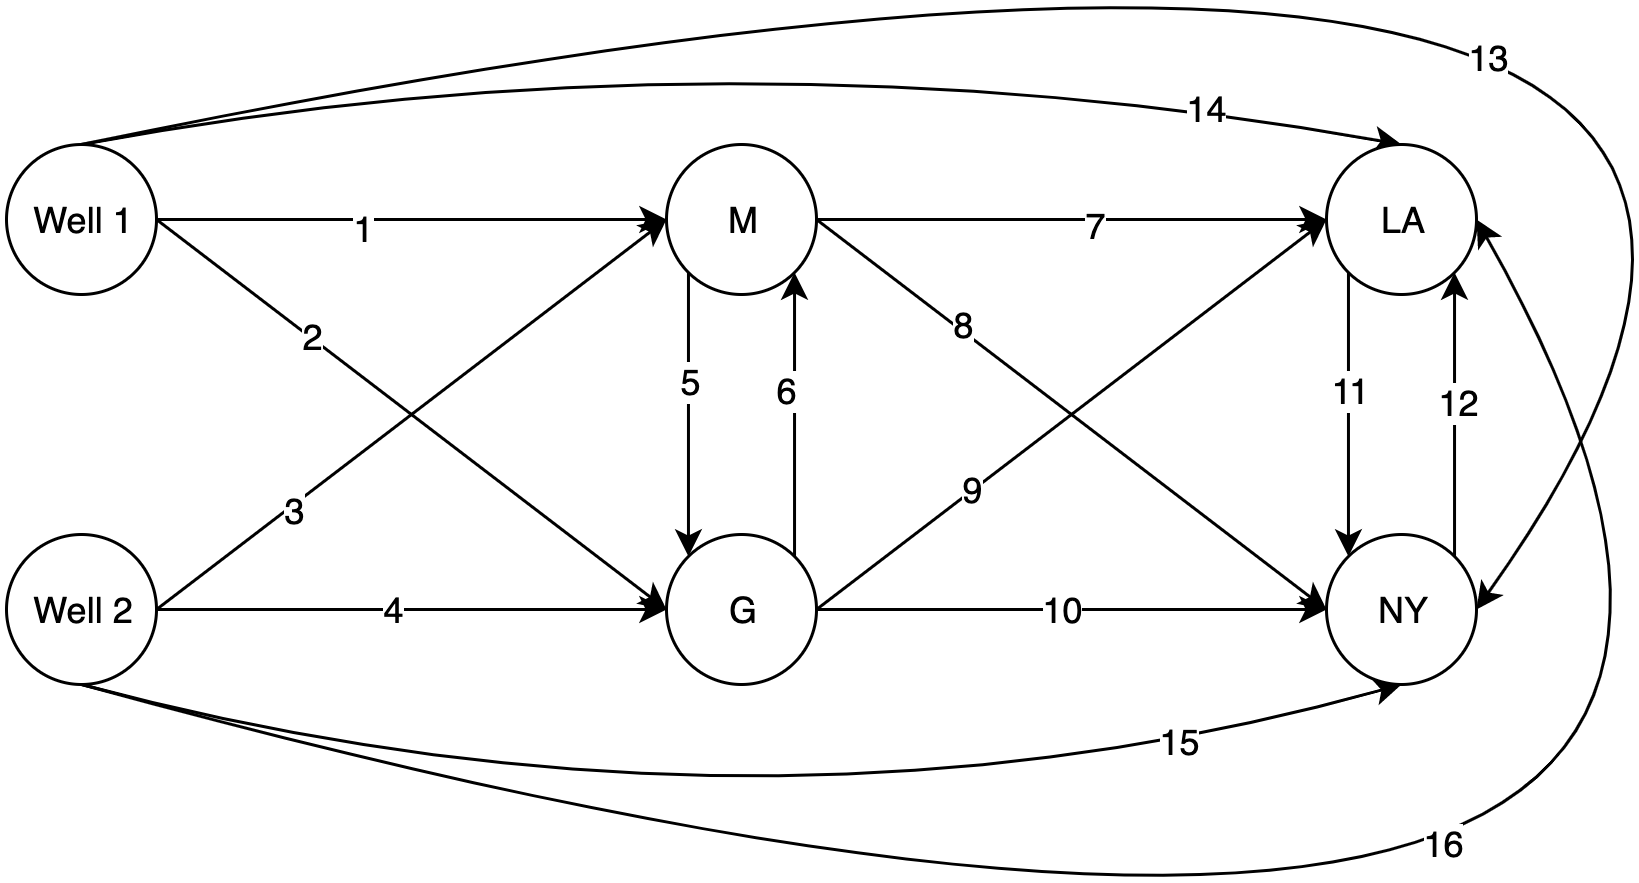
\includegraphics[width=0.9\textwidth]{hw1/hw1-prob2-graph.png}
    \caption{Network Flow of Sunco Oil Problem (labeled)}
    \label{fig:sunco_nodes}
\end{figure}

For this problem, $x_i$, the number of barrels sent via arc $i$ as labeled in Figure \ref{fig:sunco_nodes} is the \textbf{decision variables} (Unit: 1000 bbl). The \textbf{objective function} for this problem would be 
$$
\min \sum_i C_i x_i
$$
where $C_i$ is the unit shipping cost via arc $i$. 

Here we enumerate all constraints
\begin{enumerate}
\item Cleared Ports\par
Number of barrels ship into the ports must be all shipped out via outward arcs.
\begin{align*}
x_1 + x_3 + x_6 &= x_5 + x_7 + x_8 &(\text{Mobile cleared})\\
x_2 + x_4 + x_5 &= x_6 + x_9 + x_{10} &(\text{Galveston cleared})
\end{align*}

\item Demand
The number of barrels in customer location must satisfy the demand
\begin{align*}
x_7 + x_9 - x_{11} + x_{12} + x_{14} + x_{16} &\geq 170 &(\text{LA demand})\\
x_8 + x_{10} + x_{11} - x_{12} + x_{13} + x_{15} &\geq 150 &(\text{NY demand}) 
\end{align*}

\item Supply
Wells has limited supply per day. 
\begin{align*}
x_1 + x_2 + x_{13} + x_{14} &\leq 180 &(\text{Well 1 supply})\\
x_3 + x_4 + x_{15} + x_{16} &\leq 210 &(\text{Well 2 supply})
\end{align*}

\item Non-negativity
The shipping of each arc is greater or equal to zero.
$$
\forall i \in [1,...,16], x_i \geq 0
$$

\end{enumerate}

\section{Parameter Estimation}

\subsection{A Ball}\label{prob3-1}
\textbf{Decision Variable} is parameter $g$, as we are doing parameter estimation. \textbf{Objective function} is 
$$
\min \sum_t^n \norm{s(t:g) - \hat{y}_t}^2
$$
\textbf{Constraint} is only non-negativity $g \geq 0$ 

\subsection{Stock} \label{prob3-2}

\textbf{Decision Variables} are parameters $a$ and $b$. \textbf{Objective function} is 
$$
\min \sum_t^n \norm{P_X(P_Y,P_Z,t:a,b) - \hat{P_X}(t)}
$$
No \textbf{Constraints} as it is only parameters.

\section{Manufacturing Process}\label{prob4}

Decomposing the problem, we could get a general sense that three processing sequences are going on in this manufacturing process, two of which produces product A and one of which produces product B (sequence 1 for A: [1,2,4,2], sequence 2 for A, [1,2,4,3], sequence 3 for B: [1,3,4]). We define $x_i$, the input raw material to the i-th processing sequence, as the \textbf{decision variable}. Here we present a series of definitions to consolidate our model building.

\begin{enumerate}
\item Facility Sequence $sf(i, j)$ denotes the j-th facility in i-th processing sequence. For example $sf(1, 3)$ means the 3rd facility in sequence 1, which is facility 4. 
\item Sequence Running Cost $cost(i)$\par
$$
cost(i) = \sum_j c_{sf(i, j)} \frac{x_i \prod_k^{j-1} r_{sf(i, k)}}{G_{sf(i,j)}}
$$
where $c$ is the hourly cost of facility, $r$ is the recovery rate after passing a facility, $G$ is the input gallons per hour to each facility. The second term basically denotes the hours at each facility, which is the actual input gallons divided by the theoretical inputs per hour. 

As an example, calculating the cost of running procedure A through process 2 is
$$
cost(2) = 150\frac{x_2}{300} + 200 \frac{(0.9)x_2}{450} + 180\frac{(0.9)(0.95)x_2}{250} + 250 \frac{(0.9)(0.95)(0.85)x_2}{350}
$$
\item Raw material cost $raw(i)$ gives the raw material cost for each sequence depending on the types of product they produce. 
\item Facility hours $hours(f)$ is hours that f-th facility runs in all the processes. It is a bit complicated to express in mathematical terms, as some of the facility presents more than once in processes, and therefore omitted. 
\item Sequence Production $prod(i)$
$$
prod(i) = x_3\prod_j r_{sf(i, k)}
$$
As an example, the end product of B out of sequence 3 is
$$
prod(3) = (0.9)(0.85)(0.8)x_3
$$
\item Sequence Output Price $price(i)$ gives the price of A or B depending on the sequence number. 
\item \textbf{Objective Function} shows the 
$$
\max \sum_i price(i) prod(i) - cost(i) - raw(i)x_i
$$
\end{enumerate}

Here we list all the \textbf{constraints} related
\begin{enumerate}
    \item Maximum Daily Sales\par
    \begin{align*}
    prod(1) + prod(2) &\leq 1700 & (\text{Max daily sales A})\\
    prod(3) &\leq 1500 & (\text{Max daily sales B})
    \end{align*}
    \item Shipping Facility Limit \par
    \begin{align*}
    prod(1) + prod(2) + prod(3) &\leq 2500 &(\text{Total shipping limit}) 
    \end{align*}
    \item Facility Daily Hours \par
    \begin{align*}
    hours(1) &\leq 16 &(\text{Facility 1 daily hours}) \\
    hours(2) &\leq 12 &(\text{Facility 2 daily hours}) \\
    hours(3) &\leq 12 &(\text{Facility 3 daily hours}) \\
    hours(4) &\leq 16 &(\text{Facility 4 daily hours}) \\
    \end{align*}
    \item Non-negativity
    All variables greater than zero.
    
\end{enumerate}

\pagebreak

\section{Excel Model Attachments}

\begin{figure}[h]
    \centering
    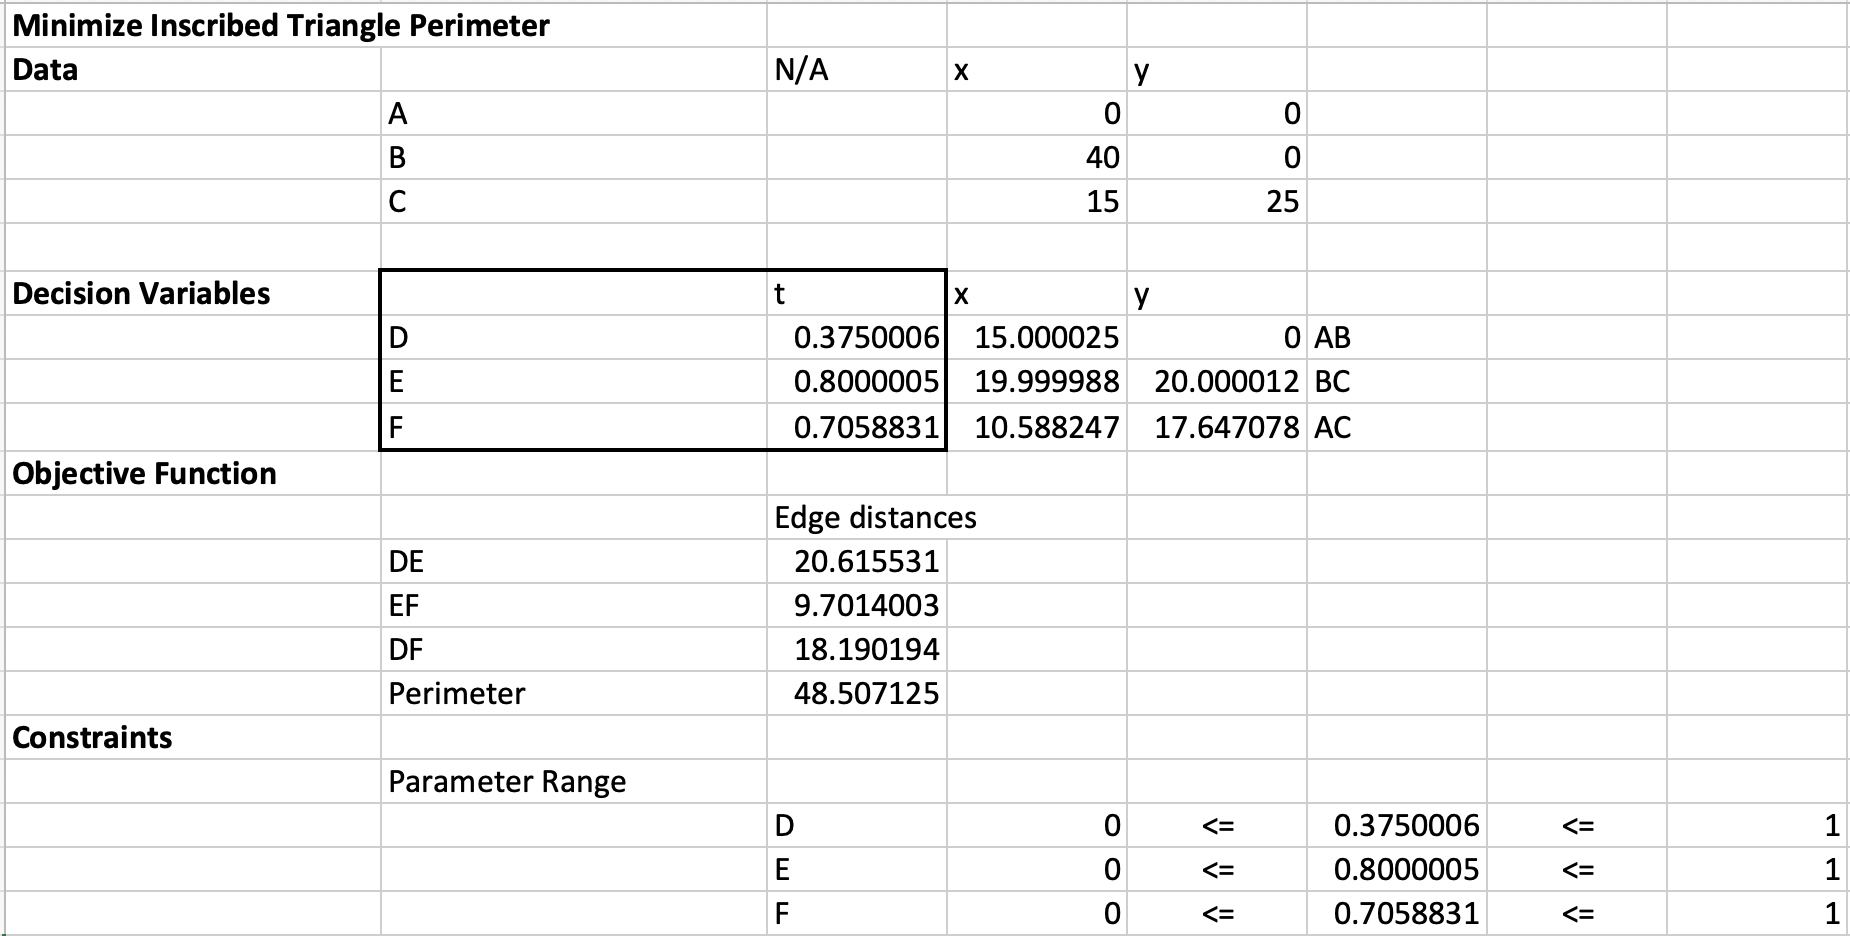
\includegraphics[width=\textwidth]{hw1/hw1-prob1.png}
    \caption{Spreadsheet Model for Problem \ref{prob1}}
    \label{fig:my_label}
\end{figure}

\begin{figure}
    \centering
    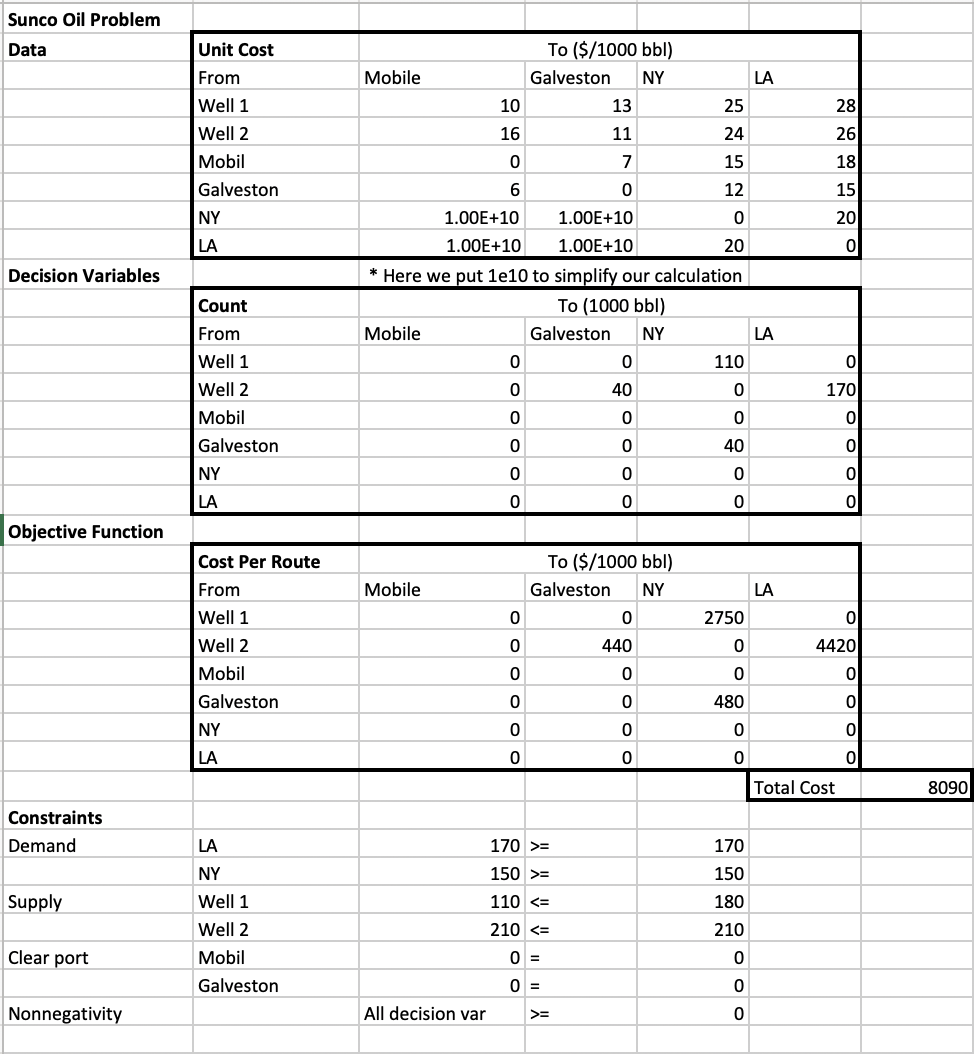
\includegraphics[width=\textwidth]{hw1/hw1-prob2.png}
    \caption{Spreadsheet Model for Problem \ref{prob2}}
    \label{fig:my_label}
\end{figure}

\begin{figure}
    \centering
    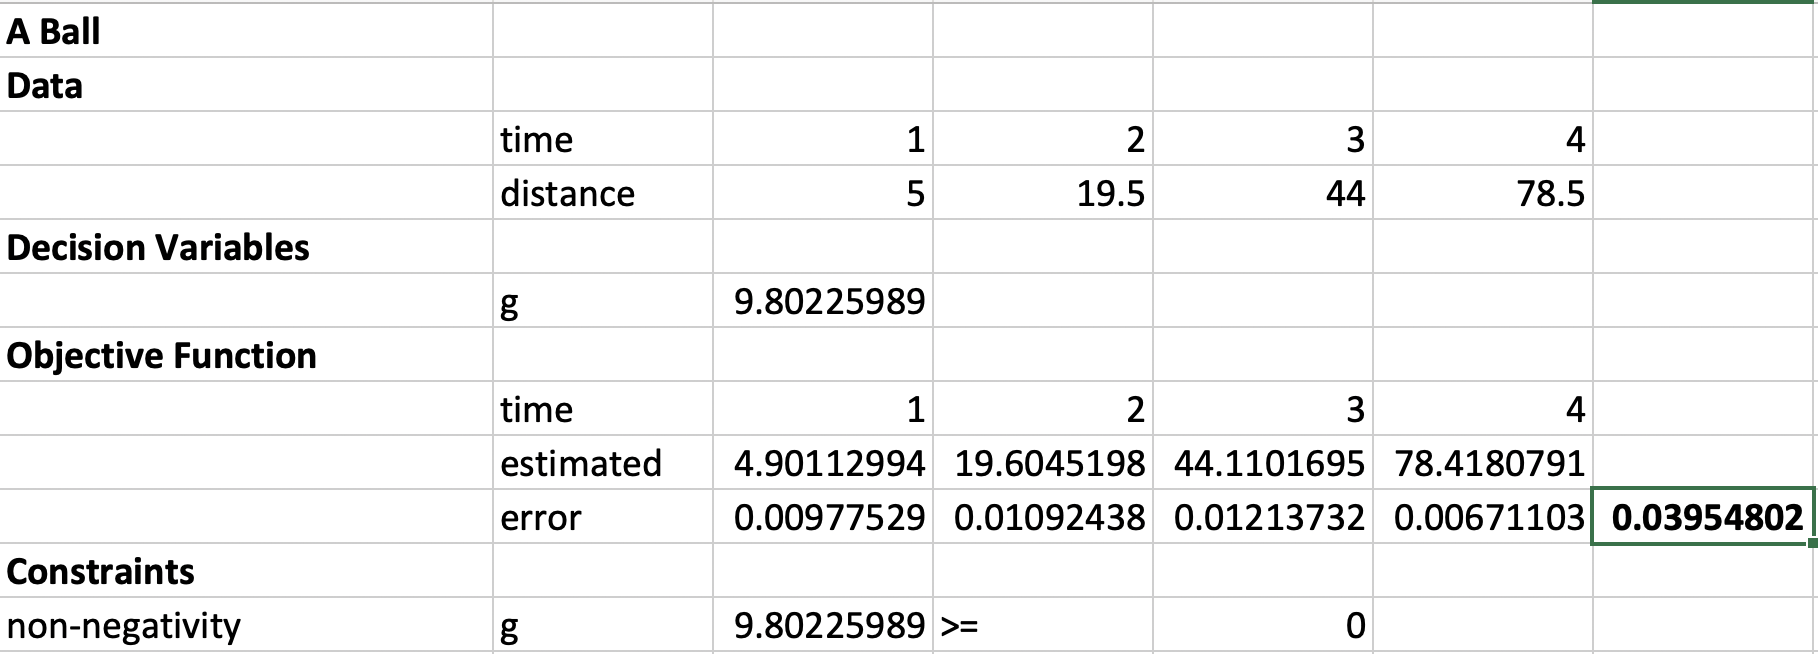
\includegraphics[width=\textwidth]{hw1/hw1-prob3-1.png}
    \caption{Spreadsheet Model for Problem \ref{prob3-1}}
    \label{fig:my_label}
\end{figure}

\begin{figure}
    \centering
    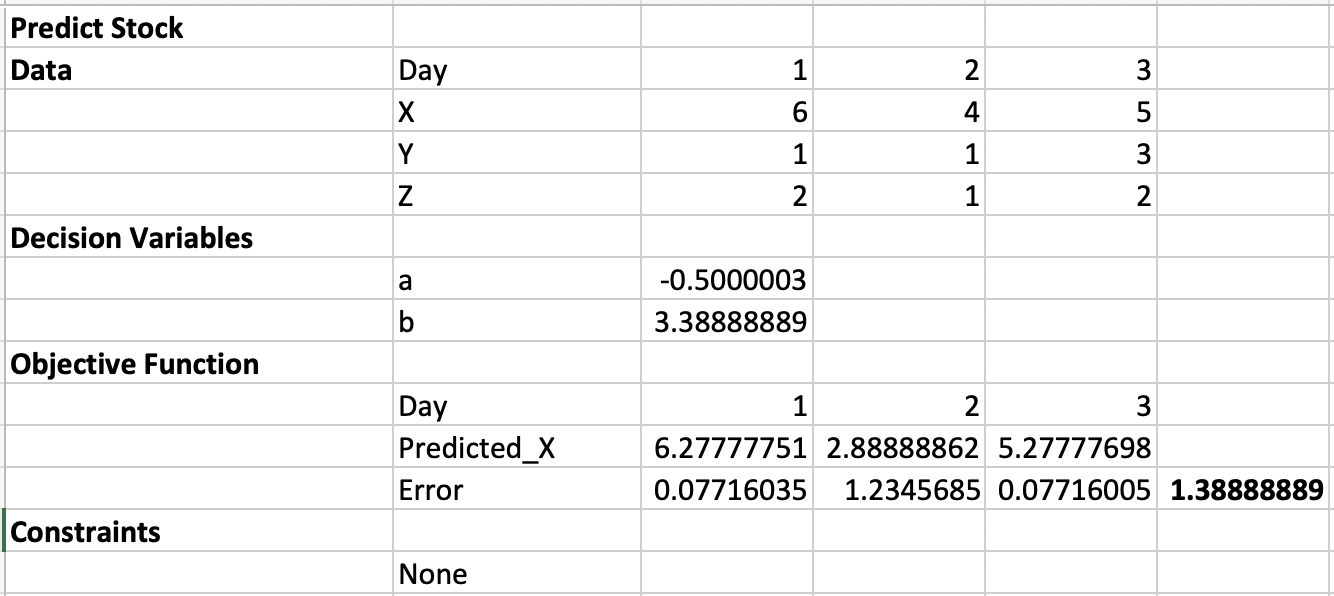
\includegraphics[width=\textwidth]{hw1/hw1-prob3-2.png}
    \caption{Spreadsheet Model for Problem \ref{prob3-2}}
    \label{fig:my_label}
\end{figure}

\begin{figure}
    \centering
    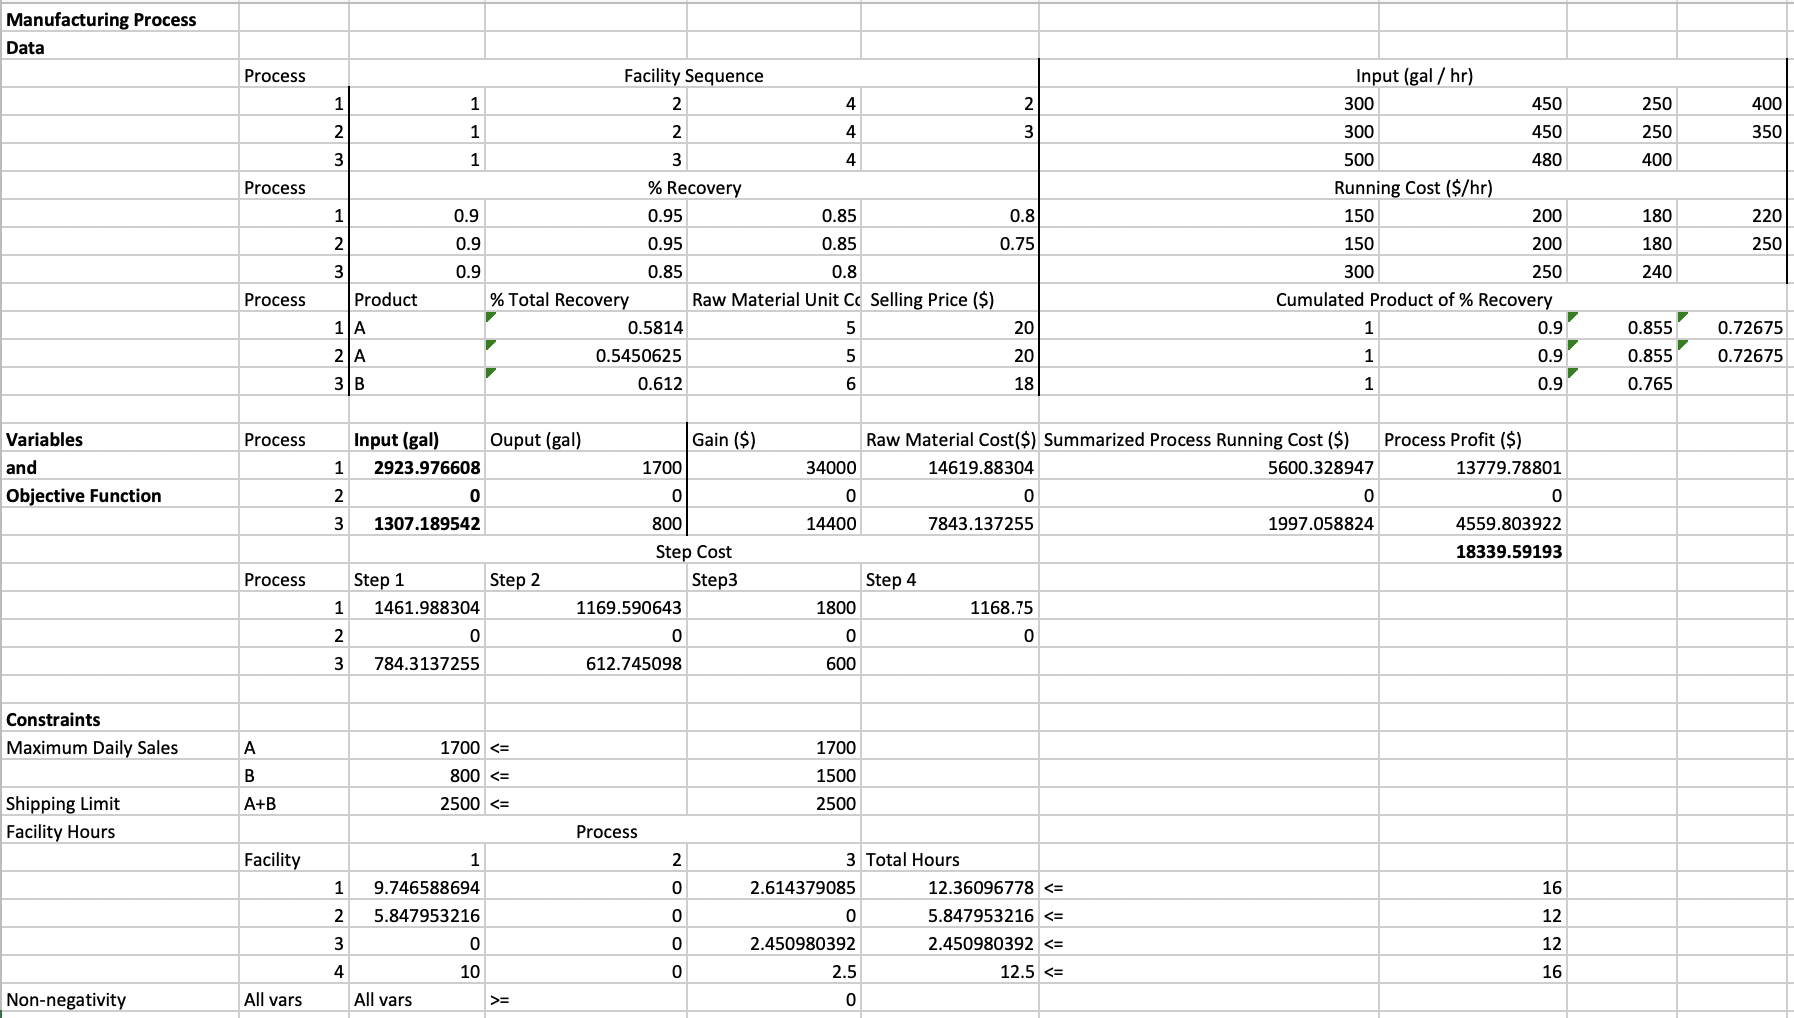
\includegraphics[width=0.9\textheight,angle=90]{hw1/hw1-prob4.png}
    \caption{Spreadsheet Model for Problem \ref{prob4}}
    \label{fig:my_label}
\end{figure}

\end{document}
